\section{The \gls{fdtd}}
The aim of this section is to give the basic of numerical simulation by using \gls{fdtd} method, such that a speaker array sound propagation can be analysed. The method of using numerical simulate will be descried, such that the method can be adapted to one or more speaker in a sound pressure field. 
The theory behind \gls{fdtd} is to solve the wave equation by a finite-difference approximation for both time and space derivatives. This make it possible to easily simulate the sound pressure and particle velocity of a speaker at any time step. One advantage of using \gls{fdtd} is that the impulse response of a specified loudspeaker can be applied to the calculation, and therefore it is possible to simulate the speaker that is used in this project. For using \gls{fdtd} with a specified speaker, all simulation have to be done in a narrow frequency band, before the simulation give a good approximation, the \gls{fdtd} can not include the hole frequency band in one simulation. A second advantage of using \gls{fdtd} is that the calculation is preformed in time domain, which benefit from that the pressure and the particle velocity at a specified time step can be analyzed directly by solving two coupled equation.\citep{fdtddaga}\\


The two equation which need to be solved is the coupled first order equation of the pressure $p$ and the particle velocity $\vec{v}$. The first formula is the Euler \autoref{fdtd_euler}, which describe the relation between the gradient for the pressure $p$ and the derivative of the particle velocity $\vec{v}$ with respect to time \autoref{fdtd_euler}. 

\begin{equation}\label{fdtd_euler}
\frac{\partial \vec{v}}{\partial t} =- \frac{1}{\rho}\vec{\triangledown }p
\end{equation}

    \startexplain
    		\explain{$\rho$ is the density of the medium }{\si{\kilo\gram\per\cubic\meter}}
        \explain{$\partial t$ is an infinitesimal time step}{\si{\second}}
        \explain{$p$ is the pressure }{\si{\pascal}}
        \explain{$\vec{v}$ is the particle velocity}{\si{\meter\per\second}}
    \stopexplain

The \autoref{fdtd_euler} is only valid with small variation of pressure. The second \autoref{fdtd_linear} is the linear continuity equation. The equation describe the relation between derivative of pressure with respect of time and the velocity gradient. They are combined by the density of the medium and the speed of sound. 

 \begin{equation}\label{fdtd_linear}
\frac{\partial p}{\partial t} =- \rho c^2 \vec{\triangledown }\vec{v}
\end{equation}

    \startexplain
    		\explain{$\rho$ is the density of the medium }{\si{\kilo\gram\per\cubic\meter}}
        \explain{$\partial t$ is an infinitesimal time step}{\si{\second}}
        \explain{$p$ is the pressure }{\si{\pascal}}
        \explain{$c$ is the speed of sound }{\si{\meter\per\second}}
        \explain{$\vec{v}$ is the particle velocity}{\si{\meter\per\second}}
    \stopexplain

Both equation are approximated by using finite difference for every point in space and time, by using a 3 dimensional grid of the space. 


\subsection{\gls{fdtd} using Cartesian grid}

The Cartesian grid for \gls{fdtd} approximation is a well known technique, and will be used in this project \citep{finiteproblems}. The Cartesian grid is using the pressure \autoref{fdtd_linear} and the particle velocity \autoref{fdtd_linear} as the unknown quantities, which have to be solved for every point in space.  A small grid is visualized in \autoref{fig:fdtd_cartesian_grid}

\begin{figure}[H]
	\centering
\begin{picture}(0,0)%
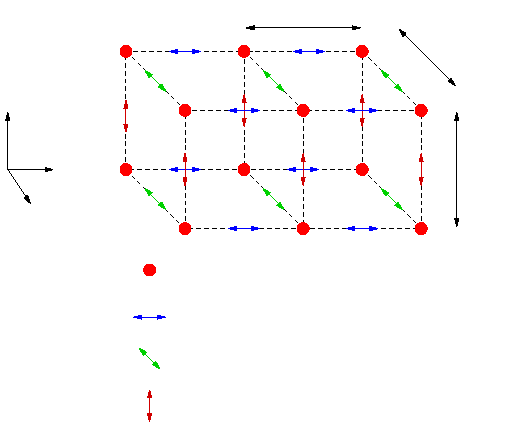
\includegraphics{fdtd_grid.pdf}%
\end{picture}%
\setlength{\unitlength}{4144sp}%
%
\begingroup\makeatletter\ifx\SetFigFont\undefined%
\gdef\SetFigFont#1#2#3#4#5{%
  \reset@font\fontsize{#1}{#2pt}%
  \fontfamily{#3}\fontseries{#4}\fontshape{#5}%
  \selectfont}%
\fi\endgroup%
\begin{picture}(3869,3327)(3541,-1288)
\put(6841,1649){$\delta y$}%
\put(3556,1244){$z$}%
\put(4006,704){$x$}%
\put(3826,344){$y$}%
\put(5806,1874){$\delta x$}%
\put(4996,-61){Pressure point}%
\put(4996,-421){Particle velocity x-direction}%
\put(4996,-781){Particle velocity y-direction}%
\put(4996,-1096){Particle velocity z-direction}%
\put(7066,704){$\delta z$}%
\end{picture}%
	\caption{A 3 dimensional example of Cartesian grid}
		\label{fig:fdtd_cartesian_grid}
\end{figure}


The grid points is build up on positions there is descried as $(i\,\delta x,j\,\delta y,k\,\delta z)$ at time $t=l\delta t$, where the time step is visualized in \autoref{fig:fdtd_transient_point}

\begin{figure}[H]
	\centering
\begin{picture}(0,0)%
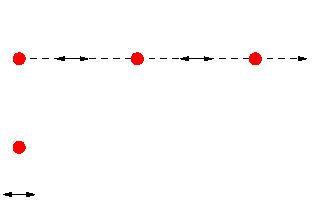
\includegraphics{fdtd_transient_point.pdf}%
\end{picture}%
\setlength{\unitlength}{4144sp}%
%
\begingroup\makeatletter\ifx\SetFigFont\undefined%
\gdef\SetFigFont#1#2#3#4#5{%
  \reset@font\fontsize{#1}{#2pt}%
  \fontfamily{#3}\fontseries{#4}\fontshape{#5}%
  \selectfont}%
\fi\endgroup%
\begin{picture}(2518,1594)(4804,-854)
\put(5266,-421){Pressure point}%
\put(5266,-781){Particle velocity}%
\put(5076,469){$(n-\frac{1}{2}) \delta t$}%
\put(5671, 29){$n \delta t$}%
\put(6456, 29){$(n+1)\delta t$}%
\put(5961,469){$(n+\frac{1}{2})\delta t$}%
\put(7246,254){$t$}%
\end{picture}%
	\caption{Transient definition points of sound $p$ pressure and particle velocity $\vec{v}$}
		\label{fig:fdtd_transient_point}
\end{figure}

$\delta x,\delta y,\delta z$ is the spatial discretization step as shown in \autoref{fig:fdtd_cartesian_grid} and $\delta t$ is the time spatial discretization step as shown in \autoref{fig:fdtd_transient_point}. $i,j,k$ is the discrete indices for the point in grid and $l$ is the discrete time index. For every axis, the component of the particle velocity have to be determined at position in \autoref{fdtd_component} at intermediant time $t=(l\pm\frac{1}{2})\delta t$ 

\begin{equation}\label{fdtd_component}
\vec{v}= \begin{bmatrix}
v_x[(i\pm \frac{1}{2})\,\delta x,j\,\delta y,k\,\delta z]\\
v_y[i\,\delta x,(j\pm \frac{1}{2})\,\delta y,k\,\delta z]\\
v_z[i\,\delta x,j\,\delta y,(k\pm \frac{1}{2})\,\delta z]
\end{bmatrix}
\end{equation}
and the pressure is determined at position $p_{(i,j,k)}^{[l+1]}$. Since the used speaker in this project is a speaker used for air operation, the medium for $\rho$ in the calculation will be air \\


The following step is done to get the linearized equation for particle velocity in Cartesian grid to any time. First \autoref{fdtd_euler} has to be rewritten to \autoref{fdtd_euler_rewrite_system}.


\begin{subequations}\label{fdtd_euler_rewrite}
\begin{alignat}{2}
-\rho_0 \frac{\partial \vec{v}}{\partial t} &=\vec{\triangledown }p \label{fdtd_euler_rewrite_1}\\
-\rho_0 \frac{\partial \vec{v}}{\partial t} &=\frac{\partial p}{\partial x}\vec{x}+\frac{\partial p}{\partial y}\vec{y}+\frac{\partial p}{\partial z}\vec{z} \label{fdtd_euler_rewrite_2}
\end{alignat}
\end{subequations}
Since $\vec{v}$ is a equation system of three inputs, the \autoref{fdtd_euler_rewrite} is splittet to a equation system \citep{Sakuma2014}.

\begin{subequations}\label{fdtd_euler_rewrite_system}
\begin{alignat}{2}
\frac{\partial p}{\partial x} &=-\rho_0 \frac{\partial v_x}{\partial t} \label{fdtd_euler_rewrite_system_1}\\
\frac{\partial p}{\partial y} &=-\rho_0 \frac{\partial v_y}{\partial t} \label{fdtd_euler_rewrite_system_2}\\
\frac{\partial p}{\partial z} &=-\rho_0 \frac{\partial v_z}{\partial t} \label{fdtd_euler_rewrite_system_3}
\end{alignat}
\end{subequations}


Next the $v_x$, $v_y$ and $v_z$ have to be differentiated with respect to $t$ and $p$ with respect to $x$, $y$ and $z$. To make it simple when differentiate with $t$ \autoref{fdtd_euler_diff_1} for all $v_x$, $v_y$ and $v_z$ only the $v_x$ is showed. The differentiation with $v_y$ and $v_z$ is similar but only the indices is at there respectively indices. When differentiate with respect to $x$, $y$ and $z$ in \autoref{fdtd_linear_diff_2} only the differentiate with respect to $x$ is done. The differentiation with respect to $y$ and $z$ is similar but only the indices is at there respectively indices \citep{Sakuma2014}.



\begin{subequations}\label{fdtd_euler_diff}
\begin{alignat}{2}
\frac{\partial v_x}{\partial t}\mid _{(i+\frac{1}{2},j,k)}^{[l]} &= \frac{(v_x)_{(i+\frac{1}{2},j,k)}^{[l+\frac{1}{2}]} -(v_x)_{(i+\frac{1}{2},j,k)}^{[l-\frac{1}{2}]}}{\delta t} \label{fdtd_euler_diff_1} \\
\frac{\partial p}{\partial x}\mid _{(i+\frac{1}{2},j,k)}^{[l]} &= \frac{p_{(i+1,j,k)}^{[l]} -p_{(i,j,k)}^{[l]}}{\delta x}  \label{fdtd_linear_diff_2}
\end{alignat}
\end{subequations}

Substituting \autoref{fdtd_euler_diff} intro \autoref{fdtd_euler_rewrite_system} and solve for $(v_x)_{(i+\frac{1}{2},j,k)}^{[l+\frac{1}{2}]}$ leads to following three \autoref{fdtd_particle_velocity}


\begin{subequations}\label{fdtd_particle_velocity}
\begin{alignat}{2}
(v_x)_{(i+\frac{1}{2},j,k)}^{[l+\frac{1}{2}]}&= (v_x)_{(i+\frac{1}{2},j,k)}^{[l-\frac{1}{2}]}-\frac{\delta t}{\rho_0 \delta x} \left( p_{(i+1,j,k)}^{[l]} -p_{(i,j,k)}^{[l]}  \right)\\
(v_y)_{(i,j+\frac{1}{2},k)}^{[l+\frac{1}{2}]}&= (v_y)_{(i,j+\frac{1}{2},k)}^{[l-\frac{1}{2}]}-\frac{\delta t}{\rho_0 \delta y} \left( p_{(i,j+1,k)}^{[l]} -p_{(i,j,k)}^{[l]}  \right)\\
(v_z)_{(i,j,k+\frac{1}{2})}^{[l+\frac{1}{2}]}&= (v_z)_{(i,j,k+\frac{1}{2})}^{[l-\frac{1}{2}]}-\frac{\delta t}{\rho_0 \delta z} \left( p_{(i,j,k+1)}^{[l]} -p_{(i,j,k)}^{[l]}  \right)
\end{alignat}
\end{subequations}
\\

The following step is done to get the linearized equation for pressure in Cartesian grid to any time. First \autoref{fdtd_linear} has to be rewritten to \autoref{fdtd_linear_rewrite_2}

\begin{subequations}\label{fdtd_linear_rewrite}
\begin{alignat}{2}
- \frac{1}{\rho_0c^2} \frac{\partial p}{\partial t} &=\vec{\triangledown }\vec{v} \label{fdtd_linear_rewrite_1}\\
- \frac{1}{\rho_0c^2} \frac{\partial p}{\partial t} &=\frac{\partial v_x}{\partial x}+\frac{\partial v_y}{\partial y}+\frac{\partial v_z}{\partial z}\label{fdtd_linear_rewrite_2}
\end{alignat}
\end{subequations}
\\


Next the $p$ have to be differentiated with respect to $t$ and $v_x$, $v_y$ and $v_z$ with respect to $x$, $y$ and $z$ respectively as done in \autoref{fdtd_linear_diff}. As in \autoref{fdtd_euler_diff} only the differentiation to $t$ and $x$ is done \citep{Sakuma2014}.



\begin{subequations}\label{fdtd_linear_diff}
\begin{alignat}{2}
\frac{\partial p}{\partial t}\mid _{(i,j,k)}^{[l+\frac{1}{2}]} &= \frac{p_{(i,j,k)}^{[l+1]} -p_{(i,j,k)}^{[l]}}{\delta t} \label{fdtd_linear_diff_1}\\
\frac{\partial v_x}{\partial x}\mid _{(i,j,k)}^{[l+\frac{1}{2}]} &= \frac{(v_x)_{(i+\frac{1}{2},j,k)}^{[l+\frac{1}{2}]} -(v_x)_{(i-\frac{1}{2},j,k)}^{[l+\frac{1}{2}]}}{\delta x} \label{fdtd_euler_diff_2}
\end{alignat}
\end{subequations}


Substituting \autoref{fdtd_linear_diff} intro \autoref{fdtd_linear_rewrite_2} and solve for $p_{(i,j,k)}^{[l+1]}$ leads to  \autoref{fdtd_pressure}




\begin{multline}\label{fdtd_pressure}
p_{(i,j,k)}^{[l+1]} = p_{(i,j,k)}^{[l]} - \rho_0 c^2 \delta t \Biggl( \frac{(v_x)_{(i+\frac{1}{2},j,k)}^{[l+\frac{1}{2}]} - (v_x)_{(i-\frac{1}{2},j,k)}^{[l+\frac{1}{2}]}}{\delta x} \\ 
+ \frac{(v_y)_{(i,j+\frac{1}{2},k)}^{[l+\frac{1}{2}]}-(v_y)_{(i,j-\frac{1}{2},k)}^{[l+\frac{1}{2}]}}{\delta y} +  \frac{(v_z)_{(i,j,k+\frac{1}{2})}^{[l+\frac{1}{2}]}-(v_z)_{(i,j,k-\frac{1}{2})}^{[l+\frac{1}{2}]}}{\delta z} \Biggr)
\end{multline}




\subsection{\gls{fdtd} grid cell size}

The chose of grid cell size for \gls{fdtd} is a critical variable which must hold some specified constrain \citep{Kunz1993}. The grid cell size have to be small enough to contain data for all specified simulated frequency, which mean that the grid cell size have to be smaller than the smallest wavelength $\lambda$. When the frequency rise the wave length is increasing. This mean the grid cell size constrain is determined by the highest frequency of interest in the \gls{fdtd} simulation. The grid cell size also have to be as a certain size such that the computation resource is kept down. The grid cell size therefore have to be chosen intelligent which \citep{Kunz1993} display one solution. After the grid cell size is chosen the Courant stability condition determined the maximum time step. The maximum time step size which will be calculated based on the grid cell size will be the used time step size because smaller time step size do not improve the accuracy generally. \\


The boundary for the lowest grid cell size is the Nyquist rate, which state that the wavelength shall at least be twice as big as the grid cell size $\delta$. Since $\delta x$, $\delta y$ and $\delta z$ have the same size only $\delta$ will be used for grid step size. The Nyquist rate is the lower boundary, but since the simulation is an approximation an is not exact and the smallest wavelength is not precise, $\delta$ have to be more than two samples per wavelength. To find a optimal grid size the grid dispersion error which relate to the wave speed through the grid will be taken intro account. The error occurs because the wave propagate slightly with different speed through the grid and this error also depending on the relative direction of the wave. The grid dispersion error is propertional to the grid cell size, which mean that the error minimized with smaller $\delta$\citep{Kunz1993}. 

Often if $ \delta \leq \frac{1}{10}\lambda_{min}$ the above constrain is met, and is therefore a good compromise between computation resource and approximation error. The grid cell size in this project is therefore as in \autoref{fdtd_delta_stepsize}

\begin{equation}\label{fdtd_delta_stepsize}
\delta x = \delta y = \delta z = \frac{1}{10} \frac{c}{f_{max}}
\end{equation}

    \startexplain
    		\explain{$\delta$ is the grid cell size }{\si{1}}
        \explain{$x$, $y$ and $z$ is the direction}{\si{1}}
        \explain{$c$ is the speed of sound}{\si{\meter\per\second}}
        \explain{$f_{max}$ is the maximum frequency in the simulation}{\si{\hertz}}
    \stopexplain
    
    
\subsection{\gls{fdtd} time step size}    
The time step size for \gls{fdtd} follows from the Courant condition \citep{Kunz1993}. The aim of the project is not to analyse the condition of Courant, this section will then explain shortly about the importers of the condition and use the condition the calculate the time step size. Consituring a plane wave, the Courant condition state that in one time step any point on the wave must not pass through more than one cell, during one time step the wave can propagate only from one cell to its nearest neighbors \citep{Kunz1993}. To determine the time step size the time step $\delta t $ can therefore be determined by the speed of light and the grid cell size as in \autoref{fdtd_time_stepsize}



\begin{equation}\label{fdtd_time_stepsize}
\delta t \leq \frac{1}{\sqrt{\frac{1}{(\delta x)^2}+\frac{1}{(\delta x)^2}+\frac{1}{(\delta x)^2} }\cdot c}
\end{equation}
        \startexplain
    		\explain{$\delta$ is the time size}{\si{1}}
        \explain{$t$ is the time indicator}{\si{1}}
        \explain{$c$ is the speed of sound}{\si{\meter\per\second}}
    \stopexplain
Making the step size smaller than \autoref{fdtd_time_stepsize} will not improve the result, in fact the equation calculate the time step size where the grid dispersion error is minimized \citep{Kunz1993}
    
\subsection{\gls{fdtd} boundary conditions}        
The meaning of the boundary condition is the condition near and at a wall. The sound wave react different on the walls than when it is propagating in free field. Wall will act like a reflecting surface, absorbing surface or both. This boundary behaviour from the wall is descried as an impedance which is frequency dependent. This have to be analysed and implemented in the simulation because the sound field will be different compare to sound field without any boundary. The frequency dependency boundary will only be a good approximation and not accurate in this project. An accurate frequency dependency model will require heavy calculation with convolution at each boundary point at each time step \citep{finiteproblems}. This kind of calculation have a high time consumption and therefore an approximation will be used. \\
The approximation in this project will then be based on the above description which use the impedance approach. \citep{FDTDmodelling} At low frequency two kind of absorbing boundary are common in real life and therefore also in simulation. this boundary is as following:

\begin{enumerate}
\item Thin absorbing boundary with respect to wavelength on a much harder background e.g wall and roof absorbers and seats.
\item Light nonstiff walls e.g. plaster walls and curtain 
\end{enumerate}


The behaviour of the first material (1) can roughly be approximated be a complex frequency dependent impedance \autoref{fdtd_thin_absorbing}

\begin{equation}\label{fdtd_thin_absorbing}
Z= Z_0+\frac{Z_{-1}}{j\omega}
\end{equation}

         \startexplain
    		\explain{$Z$ is the }{\si{1}}
        \explain{$Z_0$ is the}{\si{1}}
        \explain{$Z_{-1}$ is the }{\si{1}}
         \explain{$j$ is the complex $j$ in this context }{\si{1}}
         \explain{$\omega$ is the angle speed }{\si{1}}
    \stopexplain

The behaviour of the second material (2) can quite accurate be approximated be a complex frequency dependent impedance \autoref{fdtd_light_absorbing}

\begin{equation}\label{fdtd_light_absorbing}
Z= Z_0+j\omega M
\end{equation}

         \startexplain
    		\explain{$Z$ is the }{\si{1}}
         \explain{$M$ is the mass per unit square meter of the boundary}{\si{1}}
    \stopexplain

 \citep{finiteproblems} propose a general approximated impedance \autoref{fdtd_general_absorbing} of \autoref{fdtd_thin_absorbing} and \autoref{fdtd_light_absorbing}, which is useful for \gls{fdtd} simulation in low frequency.

\begin{equation}\label{fdtd_general_absorbing}
Z(\omega)= Z_0+\frac{Z_{-1}}{j\omega}+j\omega Z_1
\end{equation}

         \startexplain
    		\explain{$Z_1$ is the }{\si{1}}
    		\explain{$Z(\omega)$ is an expansion of the frequency impedance impedance around the frequency of interest }{\si{1}}
    \stopexplain
    
In time domain \autoref{fdtd_general_absorbing} can be expressed as the boundary condition \autoref{fdtd_boundary_absorbing}

\begin{equation}\label{fdtd_boundary_absorbing}
p(t)= Z_0v_n(t)+Z_1\int_{-\infty}^{t} v_n(\tau)d\tau +Z_1\frac{\partial u_n(t)}{\partial t} 
\end{equation}

         \startexplain
    		\explain{$p(t)$ is the acoustics pressure}{\si{\pascal}}
    		\explain{$v_n(t)$ is the component of the particle velocity orthogonal to the boundary plan}{\si{\meter\per\second}}
    \stopexplain

One arising problem in this method is that the particle velocity at the boundary, when the boundary is at plan $x=(i_0+0.5)\delta x$ which is a boundary at the $x$ velocity plan, cannot be calculated by using the pressure at $p_{(i_0+1,j,z)}$ and the same is applicable for $y$ and $z$ plan. The problem is visualized in \autoref{fig:fdtd_boundary_pressure} in 1 dimension.

\begin{figure}[H]
	\centering
\begin{picture}(0,0)%
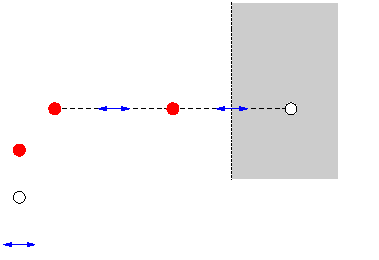
\includegraphics{fdtd_wall_reflection.pdf}%
\end{picture}%
\setlength{\unitlength}{4144sp}%
%
\begingroup\makeatletter\ifx\SetFigFont\undefined%
\gdef\SetFigFont#1#2#3#4#5{%
  \reset@font\fontsize{#1}{#2pt}%
  \fontfamily{#3}\fontseries{#4}\fontshape{#5}%
  \selectfont}%
\fi\endgroup%
\begin{picture}(2876,1975)(4534,-854)
\put(4996,-61){Pressure point}%
\put(4996,-781){Particle velocity x-direction}%
\put(4996,-421){Unknown pressure point}%
\end{picture}%

	\caption{The figure visualized a boundary plan through particle velocity plan $x$ in 1 dimension}
		\label{fig:fdtd_boundary_pressure}
\end{figure}

For solving the problem visualized in \autoref{fig:fdtd_boundary_pressure}, an asymmetric finite-difference approximation for the space derivative is used  \citep{finiteproblems}. \autoref{fdtd_boundary_absorbing} shows the asymmetric finite-difference approximation.

\begin{equation}\label{fdtd_boundary_absorbing_velocity}
\frac{\partial p}{\partial x}\mid _{(i_0+\frac{1}{2},j,k)}^{[l]} = \frac{2}{\delta x} \left( p_{(i_0+\frac{1}{2},j,k)}^{[l]}-p_{(i_0,j,k)}^{[l]} \right)
\end{equation}\\

The advance of \autoref{fdtd_boundary_absorbing_velocity} is that it only require knowledge of one nearest pressure point, but it is only valid within $\delta x$. \autoref{fdtd_boundary_absorbing} can then be used to express  \autoref{fdtd_boundary_absorbing} as function of $v_x$. Using the same procedure as in \autoref{fdtd_particle_velocity} just with plugging in \autoref{fdtd_boundary_absorbing_velocity} instead, the particle velocity at the boundary is approximated as \autoref{fdtd_boundary_eqp}

\begin{equation}\label{fdtd_boundary_eqp}
(v_x)_{(i_0+\frac{1}{2},j,k)}^{[l+\frac{1}{2}]}= (v_x)_{(i_0+\frac{1}{2},j,k)}^{[l-\frac{1}{2}]}-\frac{2 \delta t}{\rho_0 \delta x} \Biggl( 
p_{(i_0+\frac{1}{2},j,k)}^{[l]} -p_{(i_0,j,k)}^{[l]}  \Biggr)
\end{equation}

The only unknown in \autoref{fdtd_boundary_eqp} is $p_{(i_0+\frac{1}{2},j,k)}^{[l]}$ but can be founded by using \autoref{fdtd_boundary_absorbing}. $v_n$ is changed with $(v_x)_{(i_0+\frac{1}{2},j,k)}^{[l]}$ and become \autoref{fdtd_boundary_velocity}


\begin{multline}\label{fdtd_boundary_velocity}
(v_x)_{(i_0+\frac{1}{2},j,k)}^{[l+\frac{1}{2}]}= (v_x)_{(i_0+\frac{1}{2},j,k)}^{[l-\frac{1}{2}]}-\frac{2 \delta t}{\rho_0 \delta x} \Biggl( 
 Z_0(v_x)_{(i_0+\frac{1}{2},j,k)}^{[l]} \\
 +Z_1 \frac{\partial (v_x)_{(i_0+\frac{1}{2},j,k)}^{[l]}}{\partial t} +Z_{-1} \int_{-\infty}^{t} (v_x)_{(i_0+\frac{1}{2},j,k)}^{[l]}(\tau)d\tau -p_{(i_0,j,k)}^{[l]}
\Biggr)
\end{multline}

The integral in the \autoref{fdtd_boundary_velocity2} is replaced with a sum from minus infinity to $l$ in \autoref{fdtd_boundary_absorbing}.

\begin{multline}\label{fdtd_boundary_velocity2}
(v_x)_{(i_0+\frac{1}{2},j,k)}^{[l+\frac{1}{2}]}= (v_x)_{(i_0+\frac{1}{2},j,k)}^{[l-\frac{1}{2}]}-\frac{2 \delta t}{\rho_0 \delta x} \Biggl( 
 Z_0(v_x)_{(i_0+\frac{1}{2},j,k)}^{[l]} \\
+Z_1\frac{(v_x)_{(i+\frac{1}{2},j,k)}^{[l+\frac{1}{2}]}-(v_x)_{(i+\frac{1}{2},j,k)}^{[l-\frac{1}{2}]}}{\delta t}+Z_{-1} \delta t \sum_{m=-\infty}^{l} \left( (v_x)_{(i+\frac{1}{2},j,k)}^{[m+\frac{1}{2}]} \right) -p_{(i,j,k)}^{[l]}
\Biggr)
\end{multline}

The last unknown variable is the particle velocity $v_x$ at time $t=l$. To find a solution for $v_x$ at time  $t=l$  a linear interpolation between $v_x$ at time $t=(l-\frac{1}{2}) \delta t$ and $t=(l+\frac{1}{2}) \delta t$ is used \citep{finiteproblems}. The resulting particle velocity will be expressed as \autoref{fdtd_boundary_result}

\begin{multline}\label{fdtd_boundary_result}
(v_x)_{(i_0+\frac{1}{2},j,k)}^{[l+\frac{1}{2}]}= \alpha (v_x)_{(i_0+\frac{1}{2},j,k)}^{[l-\frac{1}{2}]} + \beta \frac{2 \delta t}{\rho_0 \delta x} \Biggl( 
 Z_0(v_x)_{(i_0+\frac{1}{2},j,k)}^{[l]} \\
-Z_{-1} \delta t \sum_{m=-\infty}^{l} \left( (v_x)_{(i+\frac{1}{2},j,k)}^{[m+\frac{1}{2}]} \right) -p_{(i,j,k)}^{[l]}
\Biggr)
\end{multline}


         \startexplain
    		\explain{$\alpha = \frac{1-\frac{Z_0}{Z_{FDTD}} \frac{2Z_1}{Z_{FDTD}} \delta t}{1+\frac{Z_0}{Z_{FDTD}} \frac{2Z_1}{Z_{FDTD}} \delta t}$ }{\si{1}}
    		\explain{$\beta = \frac{1}{1-\frac{Z_0}{Z_{FDTD}} \frac{2Z_1}{Z_{FDTD}} \delta t}$ }{\si{1}}
    		\explain{$Z_{FDTD} = \frac{\rho_0 \delta x}{\delta t}$ }{\si{1}}
    \stopexplain


\subsection{\gls{fdtd} stability near boundary}
A stable simulation is only guaranteed under surtain condition. Because \autoref{fdtd_boundary_result} is applied to different condition e.g. in corner of flat walls, a stable simulation is not possible in general, only with surtain condition which depend on time and grid cell size. It have be shown that the simulation is stable if $Z_0$ and $Z_{1}$ is all positive and all simulation regions if \autoref{fdtd_time_stepsize_boundary} is satisfied

\begin{equation}\label{fdtd_time_stepsize_boundary}
\delta t \leq \sqrt{\frac{2}{3}}  \left( \frac{1}{\sqrt{\frac{1}{(\delta x)^2}+\frac{1}{(\delta x)^2}+\frac{1}{(\delta x)^2} }\cdot c} \right)
\end{equation}


If $Z_{-1}$ is nonzero the time step shall also satisfy \autoref{fdtd_time_stepsize_boundary_Z_n1}

\begin{equation}\label{fdtd_time_stepsize_boundary_Z_n1}
c \delta t \leq \delta x \left(   \frac{1+\frac{2Z_1}{\rho_0 \delta x}}{1+\frac{2Z_-1 \delta x}{\rho_0 c~^2}}  \right)^{\frac{1}{2}}
\end{equation}




